\subsubsection{Datenbankmodelle und Schemata}
Ein Model in Mongoose ist ein aus einer Schemadefinition erstellter Konstruktor, aus denen Objekte instanziiert werden können. Diese Instanzen stehen in direkter Verbindung zu den jeweiligen Collections der verbundenen Datenbank und enthalten Methoden für die persistente Speicherung, Bearbeitung oder Löschung.

%TODO Konzeptioneller Aufbau
\begin{figure}[tbt]
\centering
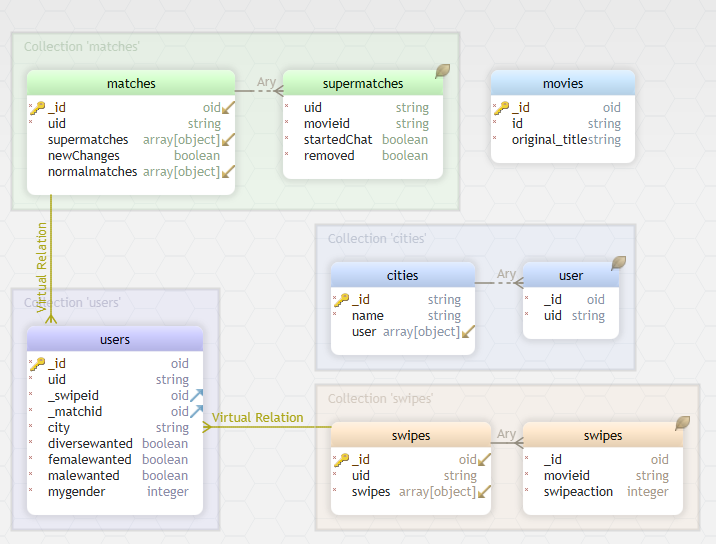
\includegraphics[width=\textwidth]{images/databasemodells.PNG}
\caption{MongoDB - Aufbau der Collections und Beziehungen}
\label{fig:databasemodells}
\end{figure}

\noindent
Listing \ref{lst:modelswipe} zeigt den Aufbau des Schemas für die Swipe-Collection. \\

\begin{lstlisting}[caption=Swipe Schema und Model, label=lst:modelswipe]
const mongoose = require('mongoose')

const swipeSchema = new mongoose.Schema({
 uid: {
  type: String,
  required: true
 },
 swipes :
 [{ movieid: { type: String },
    swipeaction: {type: Number}}]
 })

module.exports = mongoose.model('Swipe',swipeSchema)
\end{lstlisting}

\noindent
Die einzelnen Schemata wurden nach dem in Abbildung \ref{fig:databasemodells} dargestellten Aufbau für jede Collection in separate Dateien unter dem Verzeichnis '/database/models' erstellt (siehe Abbildung \ref{fig:node_structure}). Jede Datei exportiert dabei das aus dem zugehörigen Schema erzeugte Model.

\begin{figure}[tbt]
\centering
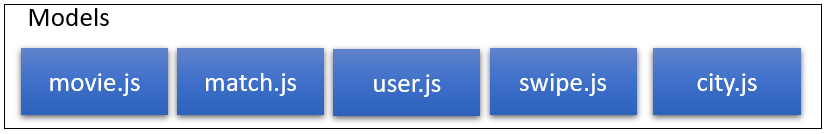
\includegraphics[width=12cm]{images/modelsstruktur.PNG}
\caption{Node.js Server - Models Struktur}
\label{fig:node_structure}
\end{figure}
